% Latex template: mahmoud.s.fahmy@students.kasralainy.edu.eg
% For more details: https://www.sharelatex.com/learn/Beamer
\documentclass[tikz]{beamer}					% Document class

\usepackage[english]{babel}				% Set language
\usepackage[utf8x]{inputenc}			% Set encoding
\usepackage{soul}
\usepackage{bm}
\usepackage{caption}
%\usepackage[demo]{graphicx}
\usepackage{subcaption}

%\mode<presentation>						% Set options
%{
%  \usetheme{default}					% Set theme
  %\usecolortheme{default} 				% Set colors
%  \usecolortheme{dolphin}%BEAMER
%  \usefonttheme{default}  				% Set font theme
%  \setbeamertemplate{caption}[numbered]	% Set caption to be numbered
%  \setbeamertemplate{frametitle}[default][left,leftskip=0mm]%BEAMER
  
%}


\mode<presentation> {

% The Beamer class comes with a number of default slide themes
% which change the colors and layouts of slides. Below this is a list
% of all the themes, uncomment each in turn to see what they look like.

%\usetheme{default}
%\usetheme{AnnArbor}
%\usetheme{Antibes}
%\usetheme{Bergen}
%\usetheme{Berkeley}
%\usetheme{Berlin}
%\usetheme{Boadilla}
% \usetheme{CambridgeUS}
%\usetheme{Copenhagen} ---
%\usetheme{Darmstadt}
%\usetheme{Dresden}
%\usetheme{Frankfurt}
%\usetheme{Goettingen}
\usetheme{Hannover}%BEAMER
%\usetheme{Ilmenau}
%\usetheme{JuanLesPins}
% \usetheme{Luebeck} ---
%\usetheme{Madrid}
% \usetheme{Malmoe} ---
%\usetheme{Marburg}
%\usetheme{Montpellier} ----
%\usetheme{PaloAlto}
%\usetheme{Pittsburgh}
%\usetheme{Rochester}
%\usetheme{Singapore}
%\usetheme{Szeged}
%\usetheme{Warsaw}

% As well as themes, the Beamer class has a number of color themes
% for any slide theme. Uncomment each of these in turn to see how it
% changes the colors of your current slide theme.

%\usecolortheme{albatross}
%\usecolortheme{beaver}
%\usecolortheme{beetle}
%\usecolortheme{crane}
\usecolortheme{dolphin}%BEAMER
%\usecolortheme{dove}
%\usecolortheme{fly}
%\usecolortheme{lily}
%\usecolortheme{orchid}
%\usecolortheme{rose}
%\usecolortheme{seagull}
%\usecolortheme{seahorse}
%\usecolortheme{whale}
%\usecolortheme{wolverine}

%% Move the title of each slide to the right of 0mm
\setbeamertemplate{frametitle}[default][left,leftskip=0mm]%BEAMER

%\setbeamertemplate{footline} % To remove the footer line in all slides uncomment this line
%\setbeamertemplate{footline}[page number] % To replace the footer line in all slides with a simple slide count uncomment this line

\setbeamertemplate{navigation symbols}{} % To remove the navigation symbols from the bottom of all slides uncomment this line
}

% Uncomment this to have the outline at the beginning of each section highlighted.
%\AtBeginSection[]
%{
%  \begin{frame}{Outline}
%    \tableofcontents[currentsection]
%  \end{frame}
%}

\usepackage{graphicx}					% For including figures
\usepackage{booktabs}					% For table rules
\usepackage{hyperref}					% For cross-referencing

% myadditions

\usepackage{mathtools}
\usepackage{cleveref}

\newcommand{\bbeta}{\bm{\beta}}
\newcommand{\hb}{\hat{\bbeta}}
\newcommand{\reals}{\mathbb{R}}
\newcommand{\OLS}{\text{OLS}}
\newcommand{\sign}{\text{sign}}

\definecolor{myc}{RGB}{127, 143, 169}


\title[]{An implementation and sensitivity study of LASSO using optimization 
methods for piecewise differentiable functions}% Presentation title

\author[]{Tathagata Basu \and M.~C.~M.~Troffaes \and J.~Einbeck}								% Presentation author
\institute[]{Durham University}			% Author affiliation
\date[]{UQOP\\18 March, 2019}									% Today's date	

\begin{document}

\setbeamercolor{structure}{fg=myc}%BEAMER

% Title page
% This page includes the information defined earlier including title, author/s, affiliation/s and the date

{
\usebackgroundtemplate{
\includegraphics[width=\paperwidth]{figures/TitleSlideBackground.png}}
\begin{frame}
  \titlepage
\end{frame}
}

{
\usebackgroundtemplate{
\includegraphics[width=\paperwidth]{figures/FrameSlideBackground.png}}

\begin{frame}{Overview}
\tableofcontents
\end{frame}
}

\section{LASSO}

{
\usebackgroundtemplate{
\includegraphics[width=\paperwidth]{figures/FrameSlideBackground.png}}

\begin{frame}{Model}
Let $\bm{X}$ be a set of predictors and $\bm{Y}$ be the corresponding response .
The linear model is given by

\begin{equation}
\label{linear_model}
\bm{Y}=\bm{X}\bbeta+\bm{\epsilon}
\end{equation}
where 
\begin{align}
\bm{Y} &\coloneqq\begin{bmatrix} y_1 \\ \vdots \\ y_n \end{bmatrix} &
\bm{X} &\coloneqq\begin{bmatrix} \bm{x}_1^T \\ \vdots \\ \bm{x}_n^T\end{bmatrix} &
\bbeta &\coloneqq\begin{bmatrix}\beta_1 \\ \vdots \\ \beta_p\end{bmatrix} &
\bm{\epsilon} &\coloneqq \begin{bmatrix}\epsilon_1 \\ \vdots \\ \epsilon_n\end{bmatrix}
\end{align}

$\epsilon_i\stackrel{i.i.d.}{\sim} N(0,\sigma^2)$ are error terms, 
$\bm{\beta}$ are regression coefficient. 
We will use $p$ and $n$ to denote the number of predictors 
and number of observations respectively, through out the presentation.
\end{frame}
}

{
\usebackgroundtemplate{
\includegraphics[width=\paperwidth]{figures/FrameSlideBackground.png}}
\begin{frame}{Regression Techniques}
\begin{block}{Ordinary Least Square}
    \begin{equation}
	\hb_{\lambda} = \arg\min_{\bbeta} \left(\frac{1}{2}\|\bm{Y}-\bm{X}\bbeta\|_2^2\right)
	\end{equation}
\end{block}
Easy to solve when $p<n$.
\begin{block}{Regularisation}
    LASSO (`Least Absolute Shrinkage and Selection Operator')
    \begin{equation}
	\hb_{\lambda} = \arg\min_{\bbeta} \left(\frac{1}{2}\|\bm{Y}-\bm{X}\bbeta\|_2^2 +\lambda \|\bbeta\|_1 \right)
	\end{equation}
\end{block}
In this case, we use optimisation techniques to get the estimates.
\end{frame}
}

\section{Optimisation}


{
\usebackgroundtemplate{
\includegraphics[width=\paperwidth]{figures/FrameSlideBackground.png}}
\begin{frame}
We explore three different optimisation techniques for this purpose.
\begin{itemize}
    \item Sub  - gradient Method
    \item Proximal Gradient Method
    \item Co-ordinate Descent Method
\end{itemize}
\end{frame}
}

\subsection{Sub-gradient Method}

{
\usebackgroundtemplate{
\includegraphics[width=\paperwidth]{figures/FrameSlideBackground.png}}
\begin{frame}{Sub-gradient Method}
\begin{block}{Sub-gradient}
    A sub-gradient of a convex function $f$ at $\beta$ is any $g\in\reals^p$
    such that for all $\gamma$ we have
    \begin{equation}
        f(\gamma) \geq f(\beta) + g(\gamma-\beta)
    \end{equation}
\end{block}
\begin{block}{Algorithm}
    We follow a similar approach like gradient descent method.
    \begin{itemize}
        \item Initial guess: $\beta^{0}$
        \item Increment step: $\beta^{(k+1)} = \beta^{(k)}-t^{(k+1)}g^{(k)}$
        \item Updating: $\beta^{(k+1)}_{*} = \arg\min\{f(\beta^{(1)}),\cdots,f(\beta^{(k+1)})\}$
    \end{itemize}
    where $t^{(k+1)}$ is the step size.
\end{block}
\end{frame}
}

{
\usebackgroundtemplate{
\includegraphics[width=\paperwidth]{figures/FrameSlideBackground.png}}
\begin{frame}{Convergence}
Convergence of the method depends on the choice of step size.
\begin{block}{Fixed step size}
    For fixed step size (i.e. $t^{(k)}=t$ for all $k=1,2,\cdots$), we have
    \begin{equation}
        \lim_{k\rightarrow \infty }f(\beta^{(k+1)}_{*}) = f^{*} + L^2t/2
    \end{equation}
    where, $|f(\beta) -f(\gamma)| \leq L\|\beta - \gamma\|_2$
\end{block}
\begin{block}{Decreasing step size}
    For decreasing step size (i.e. $\sum t^{(k)} = \infty$ and $\sum (t^{(k)})^2 <\infty$),
    we have
    \begin{equation}
        \lim_{k\rightarrow \infty }f(\beta^{(k+1)}_{*}) = f^{*}
    \end{equation}
\end{block}
where, $f^{*}$ is the optimal solution.
\end{frame}
}

\subsection{Proximal gradient Method}

{
\usebackgroundtemplate{
\includegraphics[width=\paperwidth]{figures/FrameSlideBackground.png}}
\begin{frame}{Proximal Gradient Descent Method}
\begin{block}{Decomposible function}
    Convex function $f(\beta)$ is decomposible if can be written as sum of two convex function
    \begin{equation}
        f(\beta) = g(\beta) + h(\beta)
    \end{equation}
    where $g(\beta)$ is differentiable but $h(\beta)$ is not necessarily differentiable.
\end{block}
\begin{block}{Proximal Mapping}
    The proximal mapping of $f(\beta)$ is given by:
    \begin{equation}
        prox_t(\beta) = \arg\min_{\gamma}\frac{1}{2t}\|\beta- \gamma \|^2_2 + h(\gamma)
    \end{equation}
\end{block}
We use this proximal mapping for updating.
\end{frame}
}

{
\usebackgroundtemplate{
\includegraphics[width=\paperwidth]{figures/FrameSlideBackground.png}}
\begin{frame}{Proximal Gradient Descent Method (cont.)}
\begin{block}{Algorithm}
    \begin{itemize}
        \item Initial guess: $\beta^0$
        \item Updating: $\beta^{(k+1)} = prox_t\left(\beta^{(k)}-t\nabla g(\beta^{(k)})\right)$
    \end{itemize}
\end{block}
where $t$ is stepsize.
\begin{block}{Convergence}
    Let $L$ be the Lipschitz constant of $\nabla g$, i,e, for all $\beta$, $\gamma$
    \begin{equation}
        |\nabla g(\beta)-\nabla g(\gamma)| \leq L\|\beta - \gamma\|^2_2
    \end{equation}
    Then for a fixed step-size $t$, such that, $tL\leq 1$. We have the following inequality:
    \begin{equation}
        f(\beta^{(k)}) - f^* \leq \frac{\|\beta^0 - \beta^*\|^2_2}{2kt}
    \end{equation}
\end{block}
\end{frame}
}

\subsection{Co-ordinate Descent Method}

{
\usebackgroundtemplate{
\includegraphics[width=\paperwidth]{figures/FrameSlideBackground.png}}
\begin{frame}{Co-ordinate Descent Method}
Co-ordinate Descent Method successively minimizes a multivariable 
function along each co-ordinate.
\begin{block}{Algorithm}
    \begin{itemize}
        \item Initial guess: $\beta^0$
        \item Updating: 
        \begin{align}
            \beta_1^{(k+1)} &= \arg\min_{\beta_1}
            f(\beta_1,\beta_2^{(k)},\beta_3^{(k)},\cdots,\beta_p^{(k)})\\
            \beta_2^{(k+1)} &= \arg\min_{\beta_2}
            f(\beta_1^{(k+1)},\beta_2,\beta_3^{(k)},\cdots,\beta_p^{(k)})\\
            \intertext{\vdots}
            \beta_p^{(k+1)} &= \arg\min_{\beta_p}
            f(\beta_1^{(k+1)},\beta_2^{(k+1)},\beta_3^{(k+1)},\cdots,\beta_p)
        \end{align}
    \end{itemize}
\end{block}
\end{frame}
}

{
\usebackgroundtemplate{
\includegraphics[width=\paperwidth]{figures/FrameSlideBackground.png}}
\begin{frame}{Convergence}
There are different literature for the convergence rate of co-ordinate descent algorithm
for differentiable function. However, for non-differentiable functions there are no such
global rule for convergence. In 2010, Saha \textit{et.al.} showed the convergence rate for 
the problems of the form:
\begin{equation}
    f(\beta) = g(\beta) + \lambda\|\beta\|_1
\end{equation}
where $g$ is convex and $\nabla g$ is Lipschitz with constant $L$. Then the following
inequality holds
\begin{equation}
    f(\beta^{(k)}) - f(\beta^*) = \frac{L\|\beta^0-\beta^*\|_2^2}{2k}
\end{equation}
\end{frame}
}

{
\usebackgroundtemplate{
\includegraphics[width=\paperwidth]{figures/FrameSlideBackground.png}}
\begin{frame}{Results}
We use 50 runs for a comparison between these three methods.
\begin{figure}
    \centering
    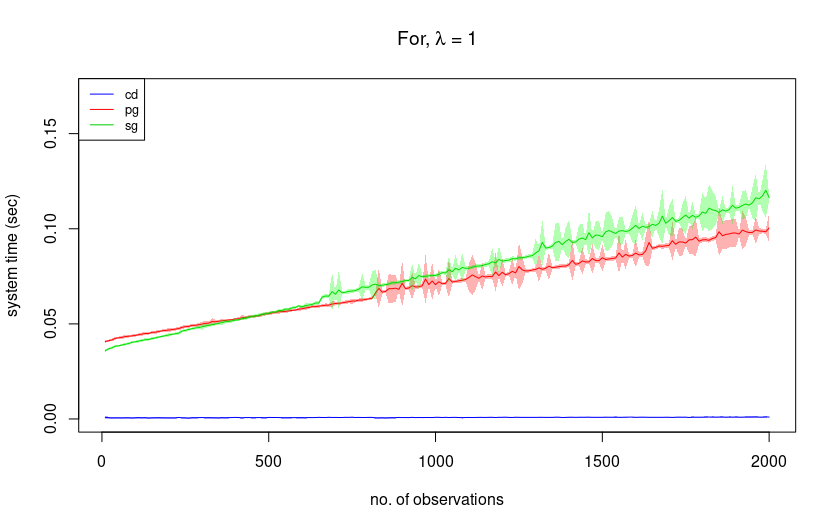
\includegraphics[width=0.7\paperwidth]{figures/obs.png}
    \caption{Runtime with respect to varying number of observations.}
\end{figure}
\end{frame}
}

{
\usebackgroundtemplate{
\includegraphics[width=\paperwidth]{figures/FrameSlideBackground.png}}
\begin{frame}{Results (Cont.)}
\begin{figure}
    \centering
    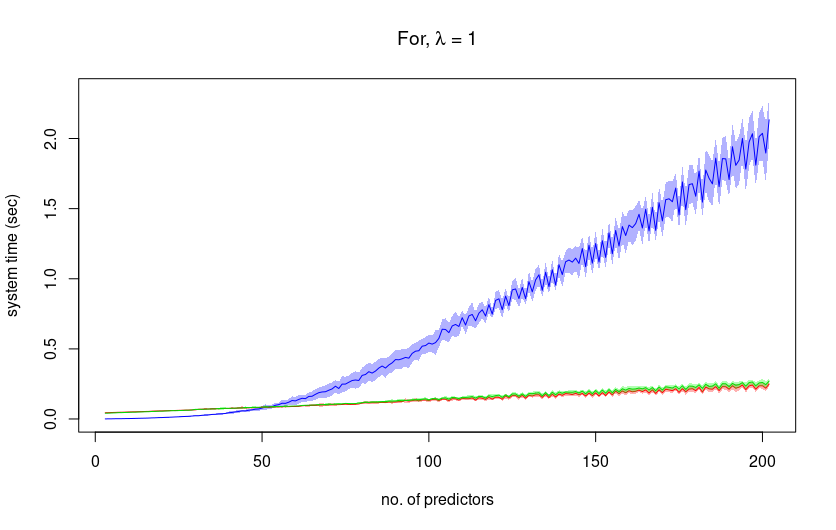
\includegraphics[width=0.7\paperwidth]{figures/pred.png}
    \caption{Runtime with respect to varying number of predictors.}
\end{figure}
\end{frame}
}

{
\usebackgroundtemplate{
\includegraphics[width=\paperwidth]{figures/FrameSlideBackground.png}}
\begin{frame}{Result (cont.)}
\begin{figure}
\begin{subfigure}{.5\textwidth}
  \centering
  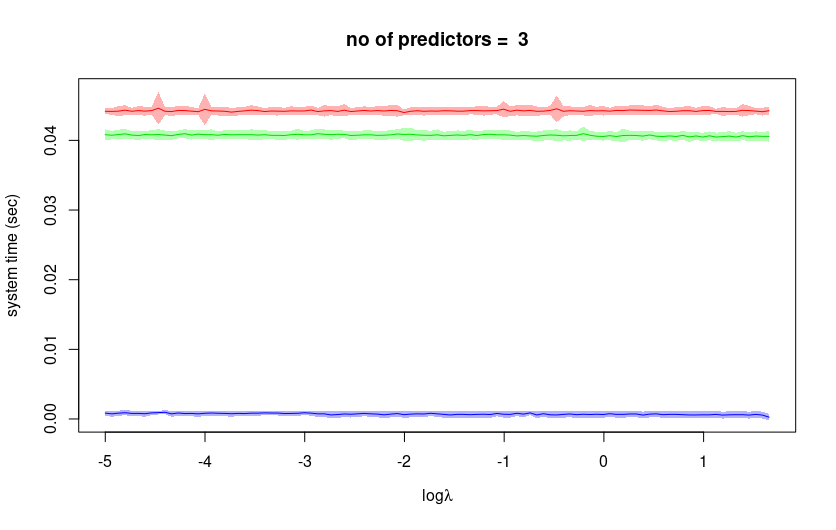
\includegraphics[width=.8\linewidth]{figures/lamb_1.png}
  \caption{runtime for 3 predictors}
\end{subfigure}%
\begin{subfigure}{.5\textwidth}
  \centering
  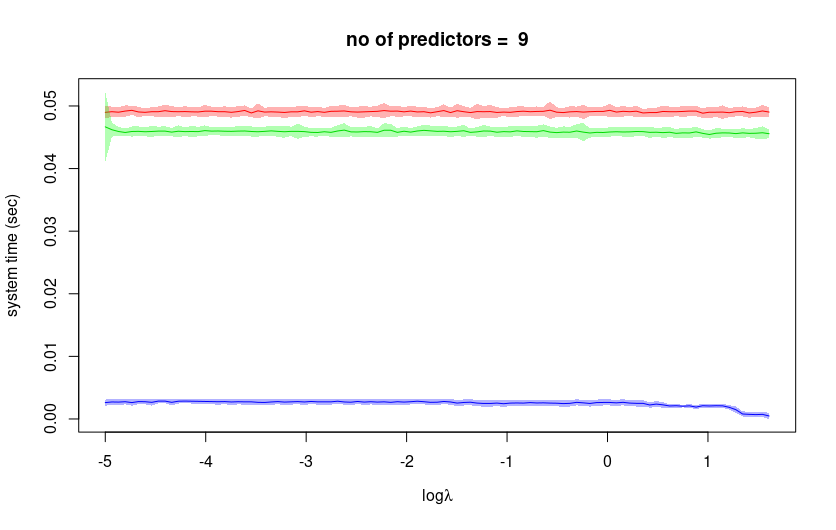
\includegraphics[width=.8\linewidth]{figures/lamb_2.png}
  \caption{runtime for 9 predictors}
\end{subfigure}
\begin{subfigure}{.5\textwidth}
  \centering
  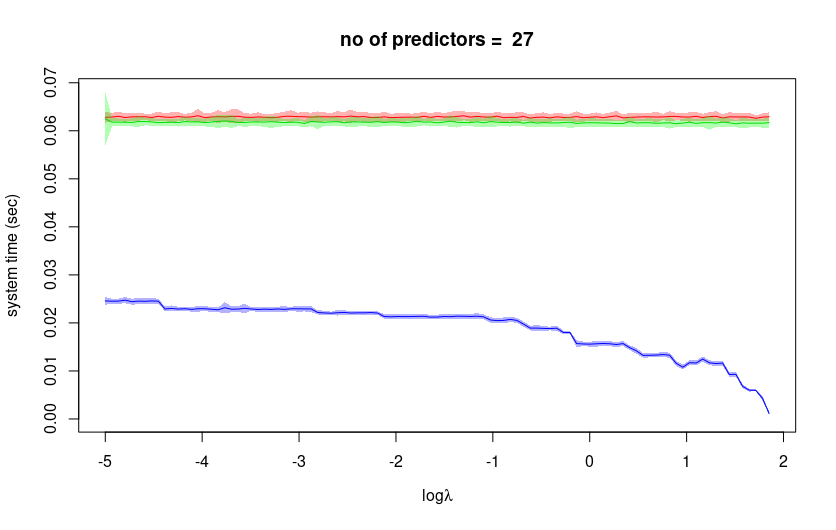
\includegraphics[width=.8\linewidth]{figures/lamb_3.png}
  \caption{runtime for 27 predictors}
\end{subfigure}%
\begin{subfigure}{.5\textwidth}
  \centering
  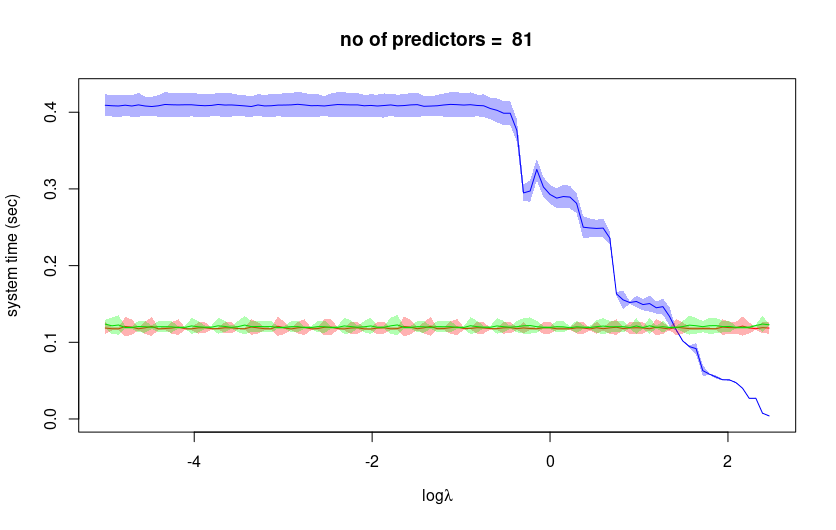
\includegraphics[width=.8\linewidth]{figures/lamb_4.png}
  \caption{runtime for 81 predictors}
\end{subfigure}
\caption{Runtime with respect to varying values of $\lambda$}
\end{figure}
\end{frame}
}

\section{Weighted LASSO}

{
\usebackgroundtemplate{
\includegraphics[width=\paperwidth]{figures/FrameSlideBackground.png}}
\begin{frame}{Weighted LASSO}
Weighted LASSO allows us to obtain differential shrinkage.
We modify the standard LASSO problem in the following way.
\begin{equation}
    \hb_{\lambda} = \arg\min_{\bbeta} \left(\frac{1}{2}\|\bm{Y}-\bm{X}\bbeta\|_2^2 +\lambda \sum_{i=1}^{p}w_i|\beta|_i \right)
\end{equation}
This allows us to incorporate our prior belief about predictors. For example,
If we want a predictor to be present in the model, then we can simply put the
corresponding weight as 0.
\begin{figure}
    \centering
    
\includegraphics[width=.4\linewidth]{figures/shrinkage.png}
    \caption{Penalty contours for different weights}
\end{figure}
\end{frame}
}
\subsection{Adaptive LASSO}

{
\usebackgroundtemplate{
\includegraphics[width=\paperwidth]{figures/FrameSlideBackground.png}}
\begin{frame}{Adaptive LASSO}
Zou introduced adaptive LASSO where he showed that careful choice of weights
results in consistency of the LASSO parameter estimates. He suggested the following
modification:
\begin{equation}
    \hb_{\lambda} = \arg\min_{\bbeta} \left(\frac{1}{2}\|\bm{Y}-\bm{X}\bbeta\|_2^2 +\lambda \sum_{i=1}^{p}w_i|\beta|_i \right)
\end{equation}
such that, $w_i = \frac{1}{|\hb_i|^{\nu}}$, where, $\nu>0$ and $\hb_i$ 
satisfies the following condition:
\begin{equation}
    \hb - \bbeta = O_p(1/\sqrt{n})
\end{equation}

\end{frame}
}

\subsection{Sensitivity Analysis}
{
\usebackgroundtemplate{
\includegraphics[width=\paperwidth]{figures/FrameSlideBackground.png}}
\begin{frame}{Sensitivity Analysis}
We introduce perturbed weights to check behavior of the predictors
under differential shrinkage.
It also allows us to incorporate our prior belief about the model and check the
robustness of the estimates with respect to it.
We modify the weighted LASSO in the following way:
\begin{equation}
    \hb_{\lambda} = \arg\min_{\bbeta} \left(\frac{1}{2}\|\bm{Y}-\bm{X}\bbeta\|_2^2 +\lambda \sum_{i=1}^{p}w_i|\beta|_i \right)
\end{equation}
such that,
\begin{equation}
    \sum_{i=1}^{p}w_i = p
\end{equation}
\end{frame}
}


{
\usebackgroundtemplate{
\includegraphics[width=\paperwidth]{figures/FrameSlideBackground.png}}
\begin{frame}{Results}
\begin{block}{Gaia Dataset}
    We did sensitivity analysis on Gaia Dataset. This set consists of 16 predictors
    which are photon bands and the response is steller temperature.
\end{block}
\begin{figure}
    \centering
    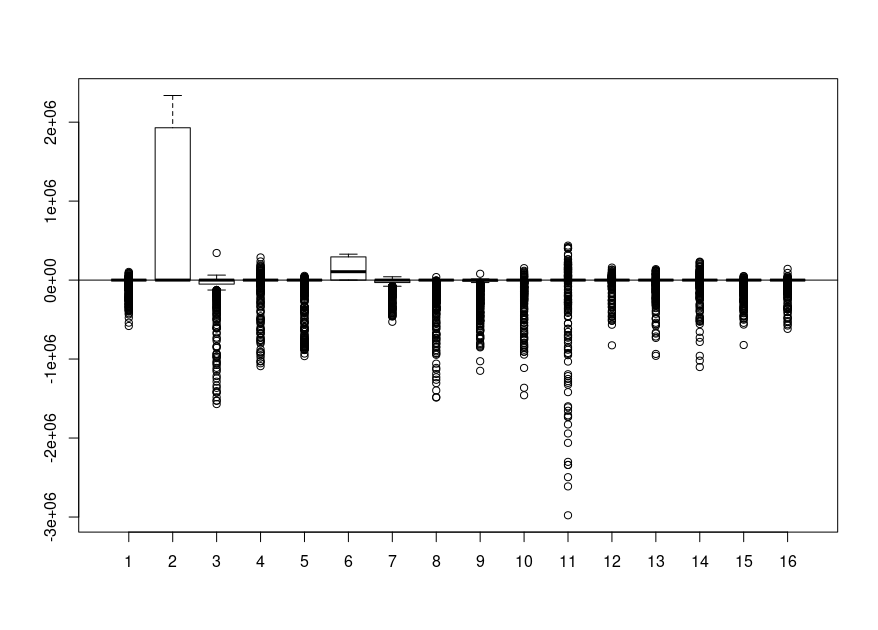
\includegraphics[width = 0.65\linewidth]{figures/sensty_gaia.png}
    \caption{Sensitivity analysis of parameter estiamtes}
\end{figure}
\end{frame}
}


{
\usebackgroundtemplate{
\includegraphics[width=\paperwidth]{figures/FrameSlideBackground.png}}
\begin{frame}{Result (cont.)}
\begin{figure}
    \centering
    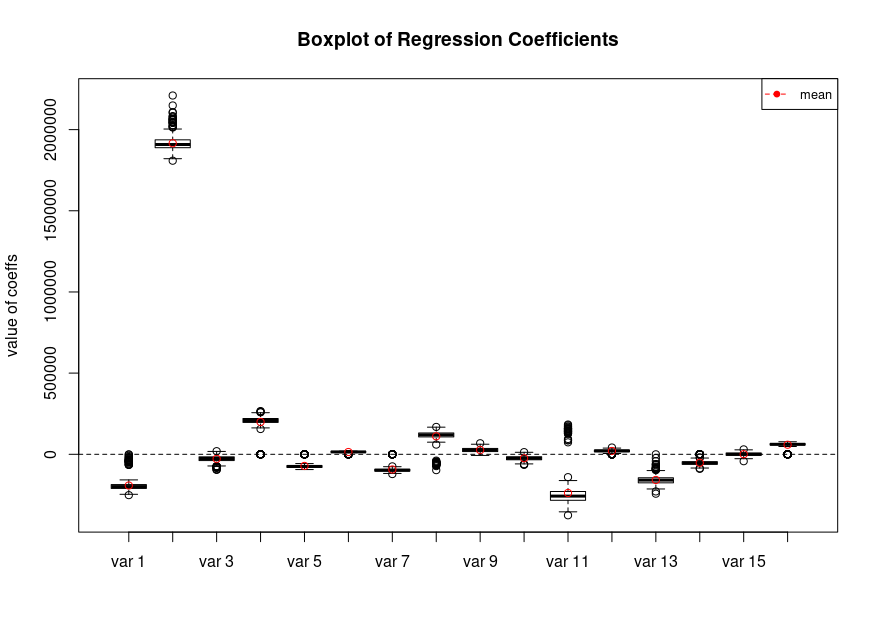
\includegraphics[width = 0.65\linewidth]{figures/bootstrap_gaia.png}
    \caption{Bootstrap estimates of parameters}
\end{figure}
This shows that the bootstrap estimates are robust w.r.t to
repeated sampling. But for differential shrinkage they tend
to shrink more.
\end{frame}
}


\section{Further Extensions}


{
\usebackgroundtemplate{
\includegraphics[width=\paperwidth]{figures/FrameSlideBackground.png}}
\begin{frame}{Further Extension}
\begin{itemize}
    \item We can further extend this to a deep search over all weights. This will allow us
    to find robust estimate using the following modification.
    \begin{equation}
        \hb_{\lambda;w} = \arg\min_{\bbeta} \left(\frac{1}{2}\|\bm{Y}-\bm{X}\bbeta\|_2^2 +\lambda \sum_{i=1}^{p}w_i|\beta|_i \right)
    \end{equation}
    then,
    \begin{align}
        \underline{\hb}_{\lambda} &= \min_{w}\hb_{\lambda;w}\\
        \overline{\hb}_{\lambda} &= \max_{w}\hb_{\lambda;w}
    \end{align}
    such that, $\sum w_i = p$ and 
    $\underline{w}_i\leq w_i\leq \overline{w}_i$ for $i=1,2,\cdots, p$.
\end{itemize}
\end{frame}
}

{
\usebackgroundtemplate{
\includegraphics[width=\paperwidth]{figures/FrameSlideBackground.png}}
\begin{frame}{Further Extension (cont.)}
\begin{itemize}
    \item We will be trying to explore the corresponding Bayesian Framework.
    
    -- Use of hierarchical model.
    \item Suitable implementation for higher number of predictors.
    
    -- Use of flag to change the optimisation technique.
\end{itemize}
\end{frame}
}


\section{Conclusion}


{
\usebackgroundtemplate{
\includegraphics[width=\paperwidth]{figures/FrameSlideBackground.png}}
\begin{frame}{Reference}
\centering
add citations!
\end{frame}
}


\end{document}
